\appendix
\renewcommand{\chaptername}{Appendix}
\chapter{Space convergence} \label{app:conv}
We report here some more convergence examples in addition to the Sin-Cos 
presented in Subsection~\ref{subsec:conv}.
%
\section{1D test}
We solve the equations~\eqref{eq:nssteadymass}--\eqref{eq:nssteadymom} over a 
one-dimensional unit domain $\Omega=(0,1)$, with the following source terms:
\begin{align}
	h &= 6x^2,\\
	f &= 12x^5 - 24\nu x - \frac{2}{\varrho} % con enableUnsymmetrizedGradient
\end{align}
so that, choosing $\varrho=1$, the analytical solution, depicted in 
Figure~\ref{fig:1dexact}, is given by
\begin{align}
\label{eq:uex1d}	u_\text{ex}(x) &= 2x^3\\
\label{eq:pex1d}	p_\text{ex}(x) &= 2-2x
\end{align}
Dirichlet boundary conditions for the velocity are applied on the whole 
boundary $\partial \Omega$ using the exact solution. The pressure is fixed at 
one point in order to match the exact solution \eqref{eq:pex1d}.
\begin{figure}
	\centering
	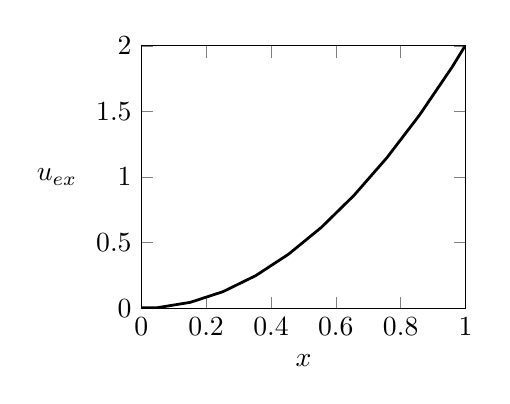
\begin{tikzpicture}
	\begin{axis}[width=0.47\textwidth, xlabel={$x$}, xmin=0, xmax=1, ymin=0, 
	ymax=2,	samples=100, ylabel={$u_\text{ex}$}, ylabel style={rotate=-90}]
	\addplot[color=black, mark=none, line width=1.0pt]{2*x*x};
	\end{axis}
	\end{tikzpicture}
%	\hskip 5pt
	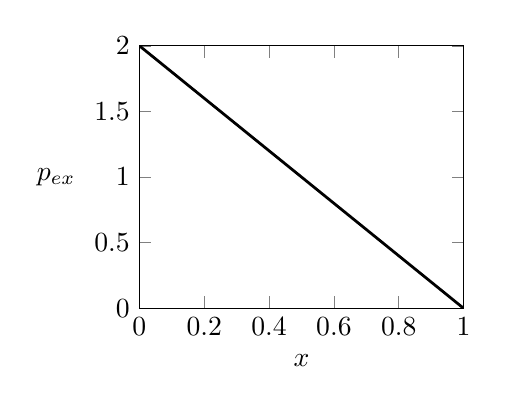
\begin{tikzpicture}
	\begin{axis}[width=0.47\textwidth, xlabel={$x$}, xmin=0, xmax=1, ymin=0, 
	ymax=2, samples=100, 
	ylabel={$p_\text{ex}$}, ylabel style={rotate=-90}]
	\addplot[color=black, mark=none, line width=1.0pt]{2*(1-x)};
	\end{axis}
	\end{tikzpicture}
	\caption[Exact solution of the 1D test]{Exact solution of the 1D test 
	\eqref{eq:uex1d}--\eqref{eq:pex1d}. On 
	the left the velocity field, on the right the pressure field.}
	\label{fig:1dexact}
\end{figure}

The problem is solved over a sequence of eight uniform grids, starting from 
4 cells and each time halving their size. Both the cases of $\nu=1$ 
and $\nu=\num{e-3}$ are considered, that correspond to $Re=1$ and $Re=\num{e3}$ 
respectively. In Figure~\ref{fig:1d_err} the errors computed are reported 
depending on the number of cells, while in 
Tables~\ref{tab:1d_lre}--\ref{tab:1d_hre} we can compare directly the 
convergence orders for the different differencing schemes.
\begin{figure}
	\centering
	\subfloat[Upwind, $Re = 1$]{
		% This file was created by matlab2tikz.
%
\definecolor{mycolor1}{rgb}{0.00000,0.44700,0.74100}%
\definecolor{mycolor2}{rgb}{0.85000,0.32500,0.09800}%
%
\begin{tikzpicture}

\begin{axis}[%
width=0.951\figwidth,
height=0.75\figwidth,
at={(0\figwidth,0\figwidth)},
scale only axis,
xmode=log,
xmin=4,
xmax=1000,
xminorticks=true,
ymode=log,
ymin=1e-06,
ymax=1,
yminorticks=true,
axis background/.style={fill=white},
legend style={at={(0.03,0.03)}, anchor=south west, legend cell align=left, align=left, draw=white!15!black}
]
\addplot [color=mycolor1, mark=x, mark options={solid, mycolor1}]
  table[row sep=crcr]{%
4	0.214116295\\
8	0.195589151\\
16	0.132868874\\
32	0.0777359686\\
64	0.0420904681\\
128	0.0219065573\\
256	0.011175991\\
512	0.00564462389\\
};
\addlegendentry{$p$}

\addplot [color=mycolor2, mark=x, mark options={solid, mycolor2}]
  table[row sep=crcr]{%
4	0.0216704604\\
8	0.0117239406\\
16	0.00417857985\\
32	0.00124123493\\
64	0.000337955248\\
128	8.81570481e-05\\
256	2.25117773e-05\\
512	5.68790627e-06\\
};
\addlegendentry{$u$}

\addplot [color=white!70!black, forget plot]
  table[row sep=crcr]{%
4	0.00025\\
1000	1e-06\\
};
\addplot [color=white!70!black, forget plot]
  table[row sep=crcr]
	\subfloat[Upwind, $Re = \num{e3}$]{
		% This file was created by matlab2tikz.
%
\definecolor{mycolor1}{rgb}{0.00000,0.44700,0.74100}%
\definecolor{mycolor2}{rgb}{0.85000,0.32500,0.09800}%
%
\begin{tikzpicture}

\begin{axis}[%
width=0.951\figwidth,
height=0.75\figwidth,
at={(0\figwidth,0\figwidth)},
scale only axis,
xmode=log,
xmin=4,
xmax=1000,
xminorticks=true,
ymode=log,
ymin=0.001,
ymax=0.190700916,
yminorticks=true,
axis background/.style={fill=white},
legend style={at={(0.03,0.03)}, anchor=south west, legend cell align=left, align=left}
]
\addplot [color=mycolor1, mark=x, mark options={solid, mycolor1}]
  table[row sep=crcr]{%
4	0.0950934111\\
8	0.0956441228\\
16	0.0633456286\\
32	0.0359064412\\
64	0.0189587968\\
128	0.009733956\\
256	0.00507474159\\
512	0.00281243348\\
};
\addlegendentry{$p$}

\addplot [color=mycolor2, mark=x, mark options={solid, mycolor2}]
  table[row sep=crcr]{%
4	0.190700916\\
8	0.161981022\\
16	0.100050412\\
32	0.0542847205\\
64	0.0273944361\\
128	0.013011169\\
256	0.00574729458\\
512	0.00230500508\\
};
\addlegendentry{$u$}

\addplot [color=white!70!black, forget plot]
  table[row sep=crcr]{%
4	0.25\\
1000	0.001\\
};
\addplot [color=white!70!black, forget plot]
  table[row sep=crcr]\\
	\subfloat[Min-Mod, $Re = 1$]{
		% This file was created by matlab2tikz.
%
\definecolor{mycolor1}{rgb}{0.00000,0.44700,0.74100}%
\definecolor{mycolor2}{rgb}{0.85000,0.32500,0.09800}%
%
\begin{tikzpicture}

\begin{axis}[%
width=0.951\figwidth,
height=0.75\figwidth,
at={(0\figwidth,0\figwidth)},
scale only axis,
xmode=log,
xmin=4,
xmax=1000,
xminorticks=true,
ymode=log,
ymin=1e-07,
ymax=0.1,
yminorticks=true,
axis background/.style={fill=white},
legend style={at={(0.03,0.03)}, anchor=south west, legend cell align=left, align=left}
]
\addplot [color=mycolor1, mark=x, mark options={solid, mycolor1}]
  table[row sep=crcr]{%
4	0.0947400829\\
8	0.0579455977\\
16	0.0306653228\\
32	0.0155606681\\
64	0.00780733847\\
128	0.00390635907\\
256	0.0019533289\\
512	0.000976635645\\
};
\addlegendentry{$p$}

\addplot [color=mycolor2, mark=x, mark options={solid, mycolor2}]
  table[row sep=crcr]{%
4	0.00558067417\\
8	0.00185644832\\
16	0.000515125253\\
32	0.000134752887\\
64	3.44440641e-05\\
128	8.70859755e-06\\
256	2.18965445e-06\\
512	5.49000176e-07\\
};
\addlegendentry{$u$}

\addplot [color=white!70!black, forget plot]
  table[row sep=crcr]{%
4	2.5e-05\\
1000	1e-07\\
};
\addplot [color=white!70!black, forget plot]
  table[row sep=crcr]
	\subfloat[Min-Mod, $Re = \num{e3}$]{
		\input{../img/l2error_test_navierstokes_1d_mm_hre}}\\
	\subfloat[Van Leer, $Re = 1$]{
		% This file was created by matlab2tikz.
%
\definecolor{mycolor1}{rgb}{0.00000,0.44700,0.74100}%
\definecolor{mycolor2}{rgb}{0.85000,0.32500,0.09800}%
%
\begin{tikzpicture}

\begin{axis}[%
width=0.951\figwidth,
height=0.75\figwidth,
at={(0\figwidth,0\figwidth)},
scale only axis,
xmode=log,
xmin=4,
xmax=1000,
xminorticks=true,
ymode=log,
ymin=1e-07,
ymax=0.1,
yminorticks=true,
axis background/.style={fill=white},
legend style={at={(0.03,0.03)}, anchor=south west, legend cell align=left, align=left}
]
\addplot [color=mycolor1, mark=x, mark options={solid, mycolor1}]
  table[row sep=crcr]{%
4	0.058505198\\
8	0.0412346964\\
16	0.0251402529\\
32	0.0139748536\\
64	0.00738268213\\
128	0.00379649657\\
256	0.00192539001\\
512	0.000969591076\\
};
\addlegendentry{$p$}

\addplot [color=mycolor2, mark=x, mark options={solid, mycolor2}]
  table[row sep=crcr]{%
4	0.00804947871\\
8	0.0022466016\\
16	0.0005523443\\
32	0.000137569802\\
64	3.46360203e-05\\
128	8.7210858e-06\\
256	2.19045006e-06\\
512	5.49050369e-07\\
};
\addlegendentry{$u$}

\addplot [color=white!70!black, forget plot]
  table[row sep=crcr]{%
4	2.5e-05\\
1000	1e-07\\
};
\addplot [color=white!70!black, forget plot]
  table[row sep=crcr]
	\subfloat[Van Leer, $Re = \num{e3}$]{
		% This file was created by matlab2tikz.
%
\definecolor{mycolor1}{rgb}{0.00000,0.44700,0.74100}%
\definecolor{mycolor2}{rgb}{0.85000,0.32500,0.09800}%
%
\begin{tikzpicture}

\begin{axis}[%
width=0.951\figwidth,
height=0.75\figwidth,
at={(0\figwidth,0\figwidth)},
scale only axis,
xmode=log,
xmin=4,
xmax=1000,
xminorticks=true,
ymode=log,
ymin=1e-06,
ymax=0.1,
yminorticks=true,
axis background/.style={fill=white},
legend style={at={(0.03,0.03)}, anchor=south west, legend cell align=left, align=left, draw=white!15!black}
]
\addplot [color=mycolor1, mark=x, mark options={solid, mycolor1}]
  table[row sep=crcr]{%
4	0.0161844304\\
8	0.00984258579\\
16	0.00351641157\\
32	0.00101607975\\
64	0.000263342669\\
128	6.34168067e-05\\
256	1.44388667e-05\\
512	3.20413694e-06\\
};
\addlegendentry{$p$}

\addplot [color=mycolor2, mark=x, mark options={solid, mycolor2}]
  table[row sep=crcr]{%
4	0.0562254093\\
8	0.020321909\\
16	0.00583980329\\
32	0.0015266502\\
64	0.000376324406\\
128	8.75670102e-05\\
256	1.88988619e-05\\
512	3.69275832e-06\\
};
\addlegendentry{$u$}

\addplot [color=white!70!black, forget plot]
  table[row sep=crcr]{%
4	0.00025\\
1000	1e-06\\
};
\addplot [color=white!70!black, forget plot]
  table[row sep=crcr]
	\caption[$L^2$-errors for the 1D problem]{$L^2$-errors for the 1D problem 
	depending on the number of cells in the grid. The grey lines are the 
	reference lines for the first-order and second-order convergence.}
	\label{fig:1d_err}
\end{figure}
\begin{table}
	\centering
	\[
	\begin{array}{c|ccc}
	\toprule
	& \text{Upwind} & \text{Min-Mod} & \text{Van Leer} \\ 
	\midrule
	p & 0.985 & 1.000 & 0.990\\
	u & 1.985 & 1.996 & 1.996\\
	\bottomrule
	\end{array}
	\]
	\caption[Convergence orders with $Re = 1$ for the 1D problem]{Convergence 
	orders with $Re = 1$ for the 1D problem. They are computed considering the 
	last two refinements of the grid.}
	\label{tab:1d_lre}
	\[
	\begin{array}{c|ccc}
	\toprule
	& \text{Upwind} & \text{Min-Mod} & \text{Van Leer} \\ 
	\midrule
	p & 0.852 & 1.501 & 2.172\\
	u & 1.318 & 2.274 & 2.356\\
	\bottomrule
	\end{array}
	\]
	\caption[Convergence orders with $Re = \num{e3}$ for the 1D 
	problem]{Convergence orders with $Re = \num{e3}$ for the 1D problem. They 
	are computed considering the last two refinements of the grid.}
	\label{tab:1d_hre}
\end{table}
%conclusions
%
\section{Kovasznay test}
We solve the equations~\eqref{eq:nssteadymass}--\eqref{eq:nssteadymom} over a 
two-dimensional domain $\Omega=(-0.5, 2) \times (-0.5,1.5)$, without any source 
term, so that, choosing $\varrho=1$, the analytical solution, depicted in 
Figure~\ref{fig:kovexact}, is given by
\begin{align}
\label{eq:uexkov} u_\text{ex}(x,y) &= 1-e^{\lambda x} \cos (2 \pi y)\\
v_\text{ex}(x,y) &= \frac{\lambda}{2\pi} e^{\lambda x} \sin (2\pi y)\\
\label{eq:pexkov}	p_\text{ex}(x,y) &= \frac{1}{2}(1 -e^{2\lambda x})\\
\lambda &= \frac{1}{2 \nu} - \sqrt{\frac{1}{4 \nu^2} + 4\pi^2},
\end{align}
as reported in \cite{test:kovasznay}.
Dirichlet boundary conditions for the velocity are applied on the whole 
boundary $\partial \Omega$ using the exact solution. The pressure is fixed at 
one point in order to match the exact solution \eqref{eq:pexkov}.
\begin{figure}
	\centering
	\subfloat{\includegraphics[width=0.5\textwidth]{kov_exact_v.png}}
	\subfloat{\includegraphics[width=0.5\textwidth]{kov_exact_p.png}}
	\caption[Exact solution of the Kovasznay test]{Exact solution of the 
	Kovasznay test \eqref{eq:uexkov}--\eqref{eq:pexkov}. On the left the 
	magnitude of the velocity field, on the 
	right the pressure field. The arrows are not scaled.}
	\label{fig:kovexact}
\end{figure}
%
\section{Angeli test}
